\documentclass[conference]{IEEEtran}
\IEEEoverridecommandlockouts

\usepackage{cite}
\usepackage{amsmath,amssymb,amsfonts}
\usepackage{algorithmic}
\usepackage{graphicx}
\usepackage{textcomp}
\usepackage{xcolor}
\usepackage{booktabs}
\usepackage[caption=false,font=footnotesize]{subfig}
\usepackage[section]{placeins}
\usepackage{float}
\usepackage{hyperref}
\def\BibTeX{{\rm B\kern-.05em{\sc i\kern-.025em b}\kern-.08em
    T\kern-.1667em\lower.7ex\hbox{E}\kern-.125emX}}
\begin{document}

\title{Automating Parametric CAD Sketch Synthesis via Sequential Decision Making\\
{\footnotesize \textsuperscript{*}Final report for AA228/CS238 (Fall 2025)}
\thanks{Course project for AA228/CS238 at Stanford University. Funded by NSF Graduate Fellowship.}
}

\author{\IEEEauthorblockN{Christopher Luey}
\IEEEauthorblockA{\textit{Department of Mechanical Engineering} \\
\textit{Stanford University}\\
luey@stanford.edu}}

\maketitle

\begin{abstract}
We automate early-stage parametric CAD sketching for planar brackets directly from structured requirement tuples. Leveraging offline trajectories from SketchGraphs, we train a sequential decision-making policy to construct geometry primitive-by-primitive. A major challenge in valid sketch generation is the ambiguity of partial graphs; standard imitation learning often yields over-confident, topologically invalid predictions. To address this, we propose a fine-tuning stage using Conservative Q-Learning (CQL) that penalizes out-of-distribution actions. We curate a bracket-focused dataset of 299 sketches and benchmark our approach against a standard Behavior Cloning (BC) baseline. Results show that CQL fine-tuning improves next-primitive accuracy by 4.4\% (from 63.0\% to 67.4\%) and reduces Expected Calibration Error (ECE) by 35\% (from 0.20 to 0.13) compared to the baseline. Visual rollouts confirm that the risk-aware policy respects orthogonal design intent while accurately signaling uncertainty at ambiguous geometric features.
\end{abstract}

\begin{IEEEkeywords}
CAD automation, offline reinforcement learning, conservative Q-learning, uncertainty calibration, SketchGraphs
\end{IEEEkeywords}

\section{Introduction}
Turning requirement tables into parametric CAD sketches is manual and error-prone. A core difficulty is that sketch construction is ambiguous: a single corner requirement could validly be satisfied by a sharp intersection (Lines) or a fillet (Arc). This "one-to-many" mapping from requirements to geometry creates a significant challenge for automation. Existing generative models often ignore this multi-modality, producing "average" geometry that breaks downstream constraint solvers.

Specifically, when a model is uncertain, it may output a mean prediction that satisfies neither option (e.g., a curve that is neither a valid line nor a valid arc). In an interactive setting, this is acceptable, but for offline automation, the system must be \textit{reliable}. It should either generate a valid construction or explicitly flag its uncertainty. We target the automation of this early-stage sketching by framing it as a sequential decision problem where the policy must not only predict the next primitive but also quantify its uncertainty.

Our contributions are: (1) a bracket-focused subset of SketchGraphs with clear geometric filters; (2) a sequential behavior cloning (BC) policy with calibrated Gaussian heads; (3) a conservative Q-learning (CQL) fine-tuning stage that penalizes risky actions; and (4) a comparative evaluation showing that risk-aware training significantly improves calibration and accuracy over the BC baseline. Code is available at \url{https://github.com/ChristopherLuey/Decision-Making-Final}.

\section{Related Work}

\subsection{Parametric CAD Generation}
SketchGraphs \cite{SketchGraphs2020} established large-scale relational CAD data, enabling the first wave of deep learning for CAD. Early approaches used autoregressive transformers to predict tokens, treating geometry as language. However, these models often struggle with the continuous nature of metric constraints. Fusion 360 Gallery \cite{Willis2021Fusion360} demonstrated programmatic CAD reconstruction with strong solver coupling, but this requires an expensive "solver-in-the-loop" during inference. DeepCAD (Wu et al., 2021) approached the problem from 3D point clouds, but such voxel-based methods lack the editability and topological validity required for engineering design. Our approach bridges this gap by operating in the parametric domain (like SketchGraphs) but enforcing reliability through offline RL principles (unlike standard autoregressive models).

\subsection{Offline RL for Design Reliability}
Offline Reinforcement Learning is typically applied to robotics or control tasks where online data collection is dangerous. We adapt it here for \textit{generative design reliability}. The core insight is that "hallucinating" invalid CAD geometry is analogous to a robot crashing: it is a failure mode we want to actively penalize. Conservative Q-learning (CQL) \cite{Kumar2020CQL} provides a mechanism to do this by learning a lower bound on the value function, effectively suppressing actions that lie outside the support of the training data. By combining this with decision-making under uncertainty principles \cite{Kochenderfer2022}, we create a sketcher that explicitly trades "creativity" for "caution."

\section{Dataset and Task Formulation}
Each trajectory begins with a requirement tuple (span, flange height, thickness, hole pattern) and a ground-truth construction sequence of primitives (Line, Arc, Circle, Point) plus constraints. We treat sketch generation as a partially observable Markov decision process (POMDP).

\textbf{State Space:} The policy observes the requirement tuple $R$ and the partial sketch graph $G_t$ constructed so far.
\textbf{Action Space:} The action $a_t$ factorizes into a primitive type (Line, Arc, Circle, Point) and continuous parameters (endpoints, centers, radii).

We start from 5{,}000 SketchGraphs validation trajectories and enforce "bracket heuristics": orthogonal spans, at least one circular feature (for bolt holes), 3--12 primitives, and at most three loops. This filters out decorative or non-functional sketches, retaining 299 high-quality examples.

Figure~\ref{fig:dataset} and Figure~\ref{fig:distribution} characterize this subset. The action space is heavily skewed toward Lines and Coincident constraints, reflecting the rectilinear nature of brackets. This class imbalance makes calibration difficult for standard supervised learning, as the model learns to blindly predict "Line" to minimize loss.

\begin{figure}[H]
    \centering
    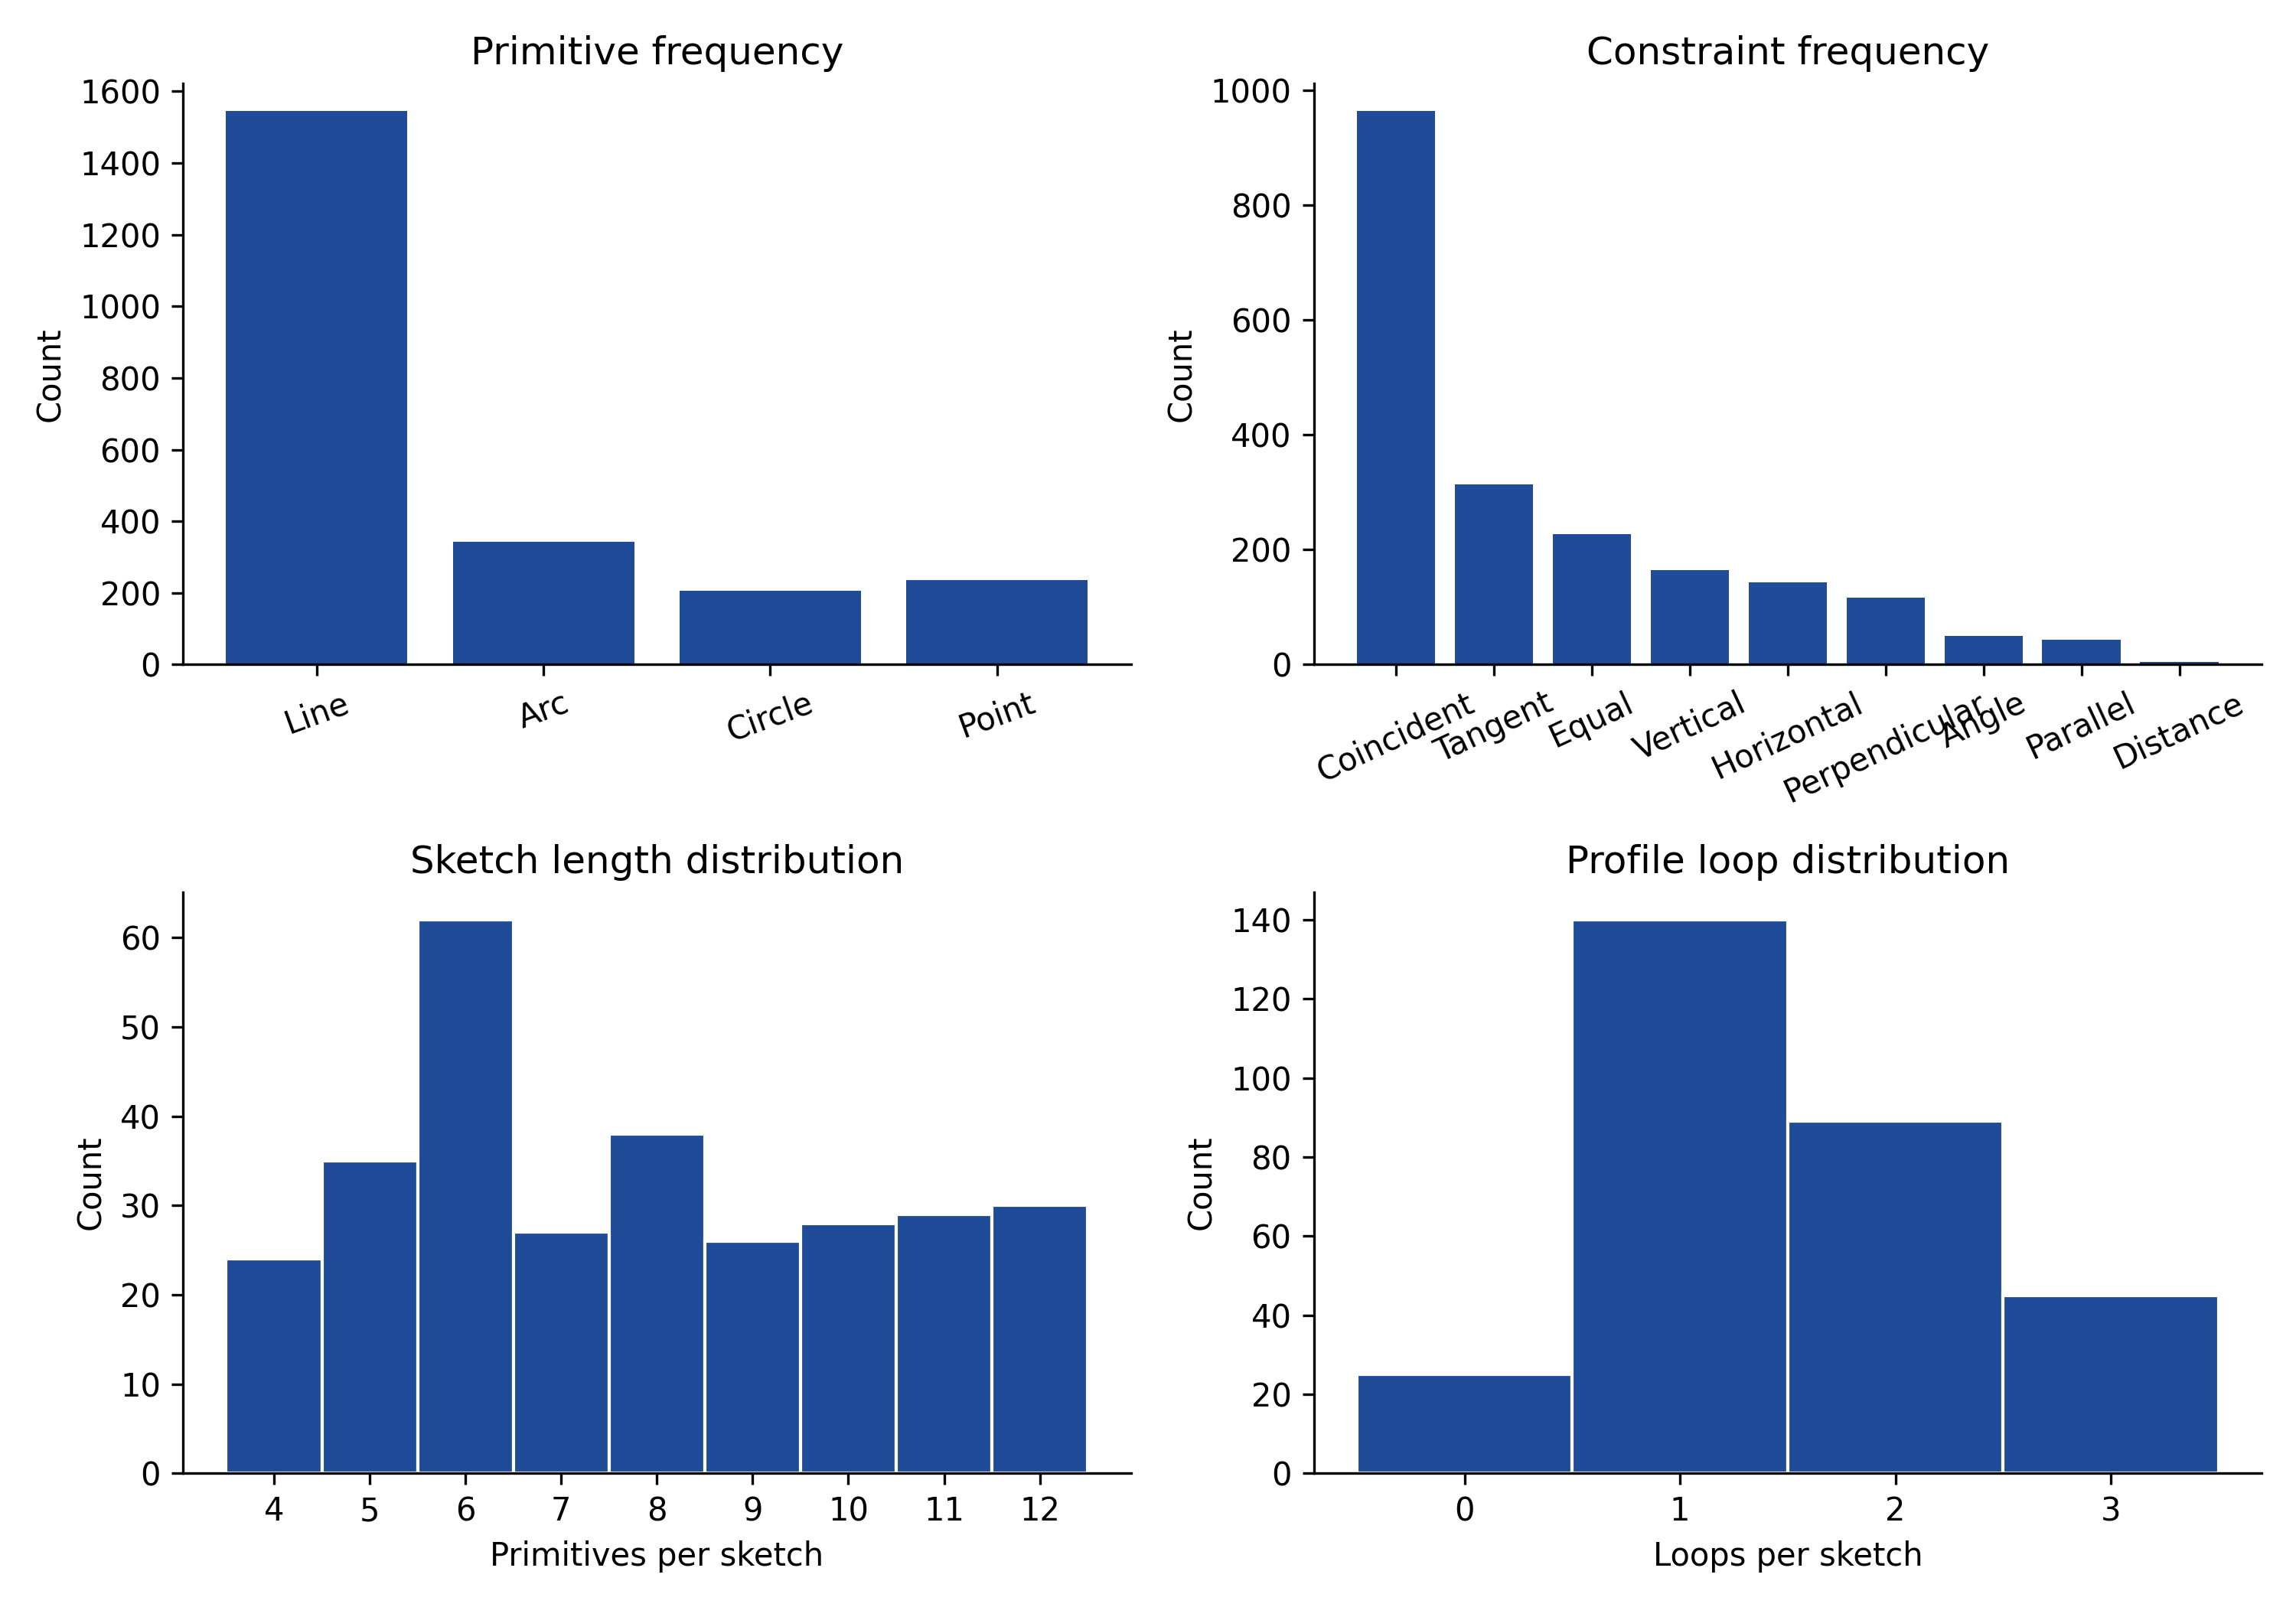
\includegraphics[width=\linewidth]{figures/dataset_overview.png}
    \caption{Dataset overview. Top: The action space is dominated by Lines and Coincident/Tangent constraints, mirroring standard bracket construction. Bottom: Sketch length and loop count distributions show the complexity range (mostly 1-2 loops).}
    \label{fig:dataset}
\end{figure}

\begin{figure}[H]
    \centering
    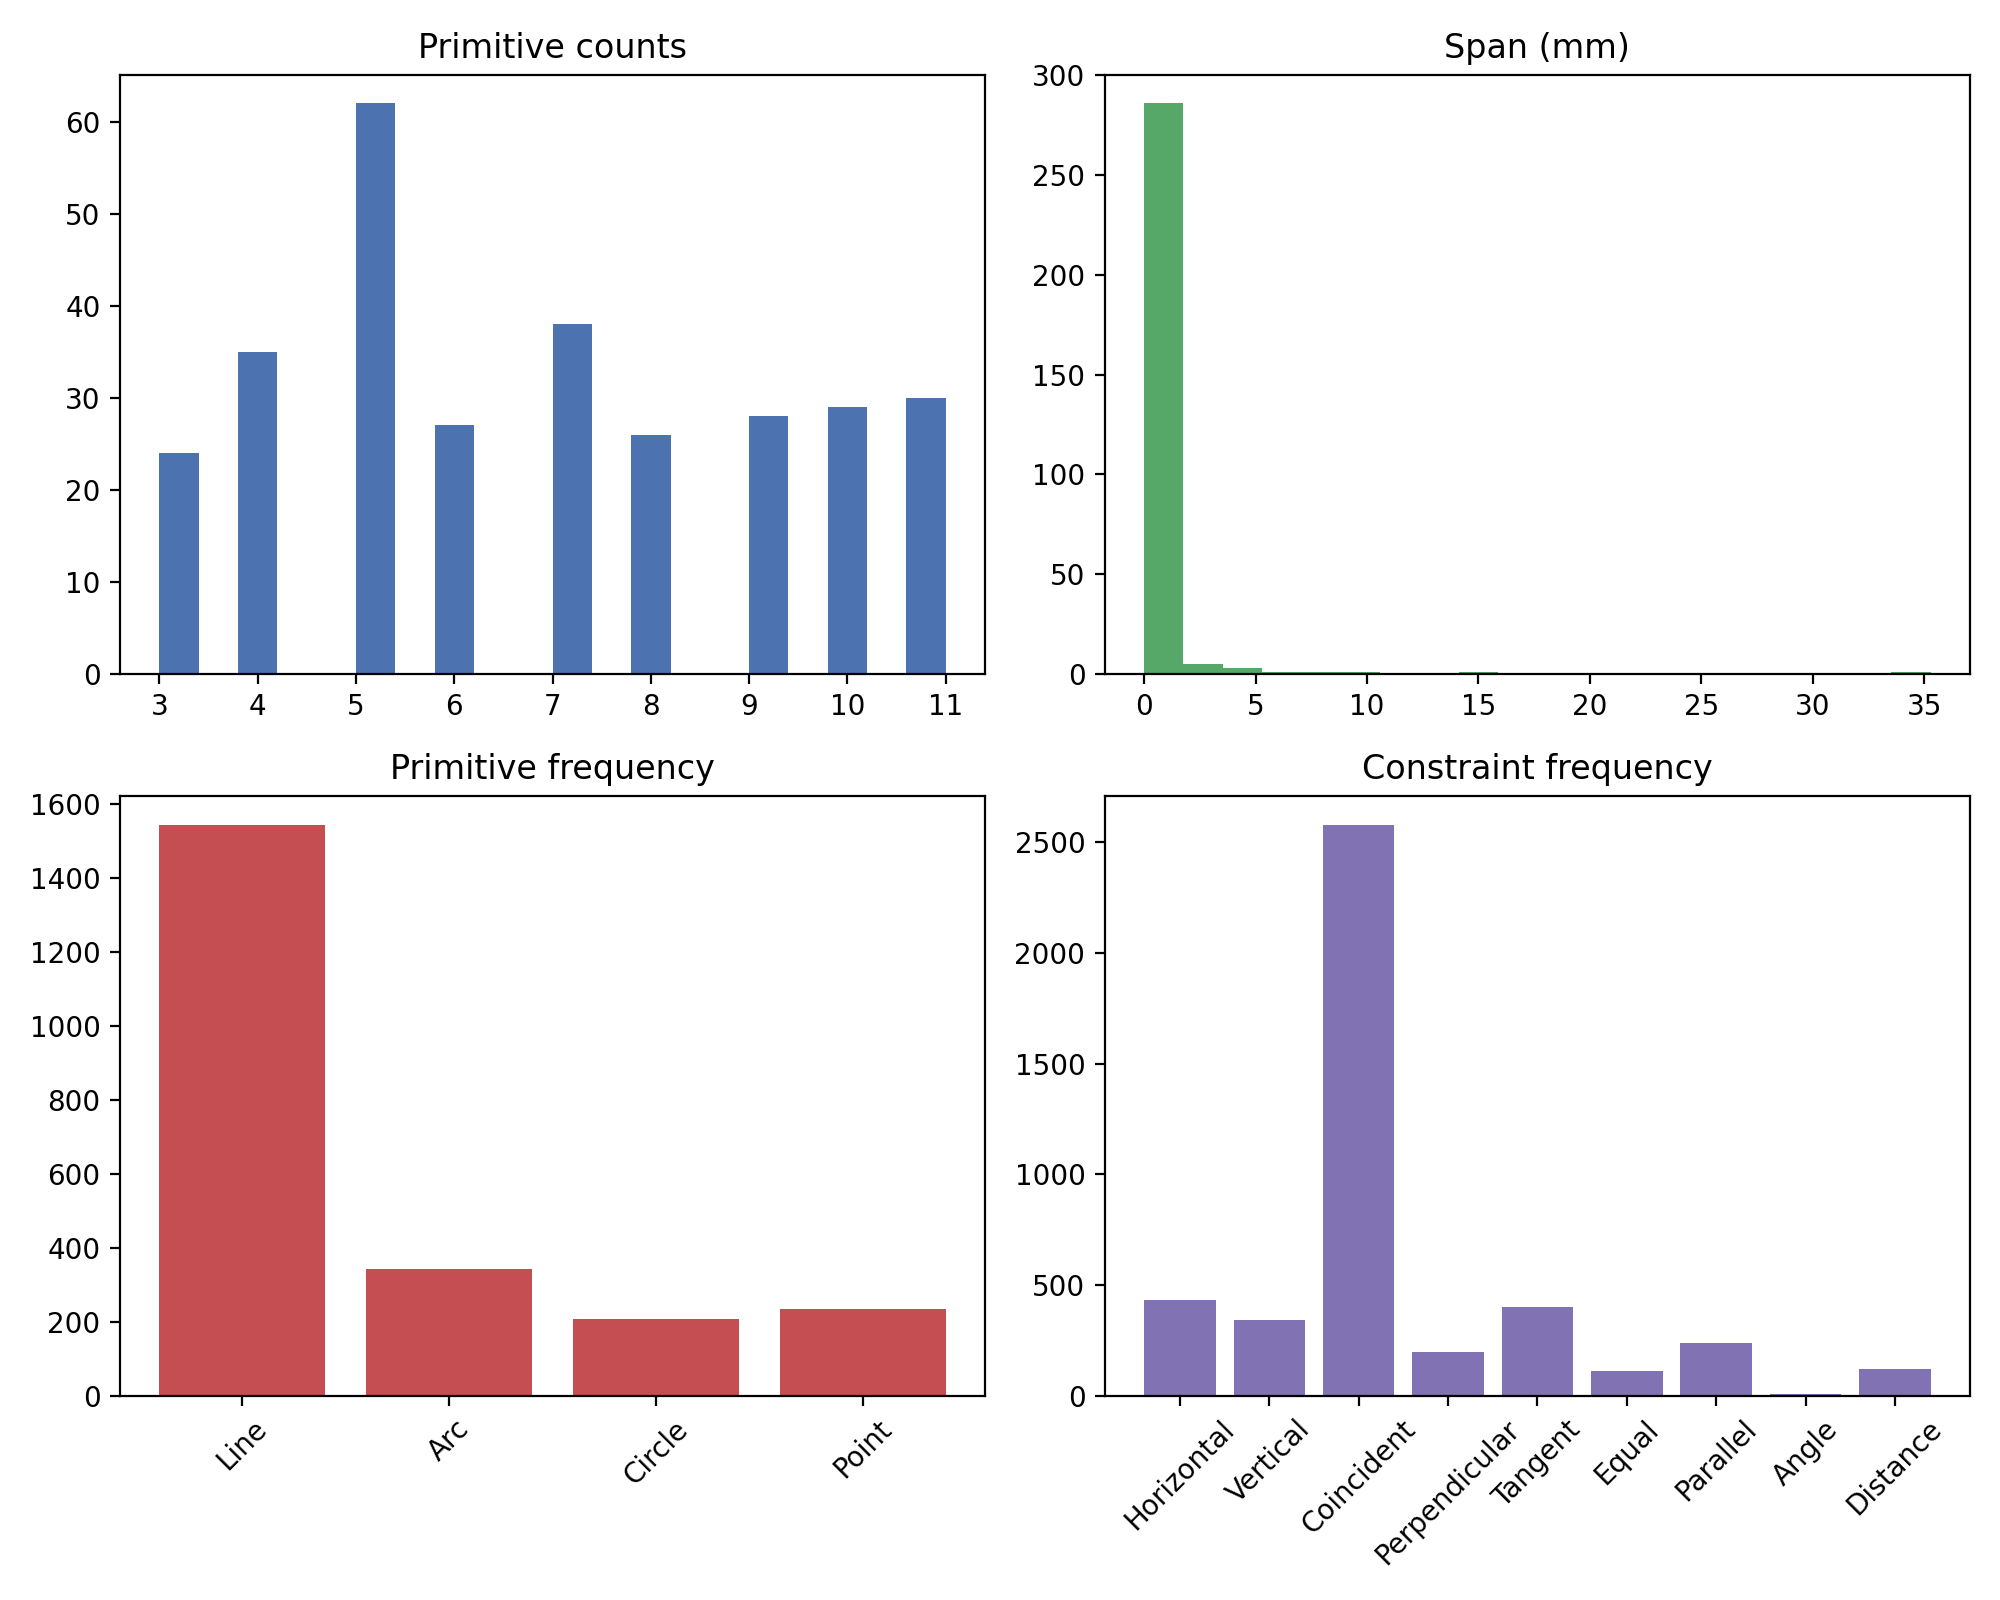
\includegraphics[width=0.9\linewidth]{figures/dataset_distribution.png}
    \caption{Detailed distribution of primitive counts (left) and loop counts (right) in the filtered dataset. We focus on sketches with 3-12 primitives to ensure tractable but non-trivial construction tasks.}
    \label{fig:distribution}
\end{figure}

\section{Methodology}

\begin{figure*}[!t]
\centering
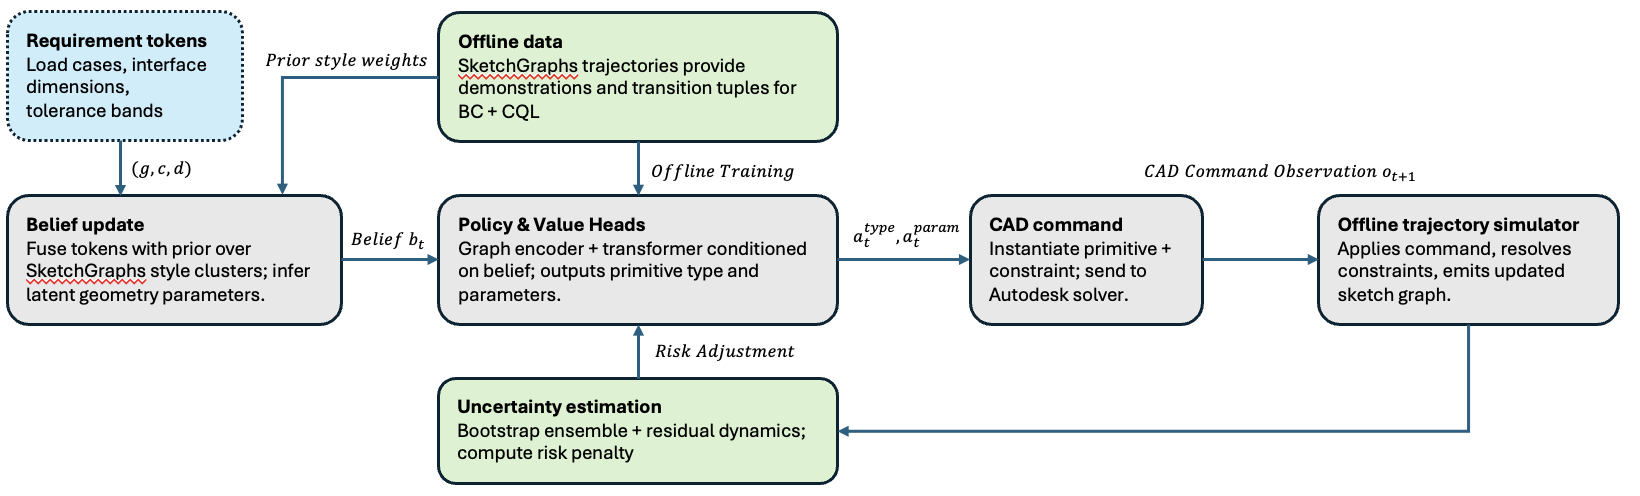
\includegraphics[width=0.9\linewidth]{figures/flowchart.png}
\caption{System Architecture. The pipeline begins with requirement tokens (top left) which are fused with a prior over style clusters to form a belief state. The policy (center) outputs primitive types and parameters, conditioned on this belief. A risk-aware fine-tuning stage (CQL) penalizes out-of-distribution actions. The offline trajectory simulator (right) updates the sketch graph state $G_{t+1}$ for the next step.}
\label{fig:flowchart}
\end{figure*}

\subsection{Behavior Cloning (Stage 1)}
We first train a Behavior Cloning (BC) policy $\pi_\theta(a|s)$ to maximize the likelihood of the expert actions in the dataset $\mathcal{D}$. The architecture uses a Gated Recurrent Unit (GRU) with 128 hidden units to encode the sequence history, and a 2-layer MLP to embed the requirements. The output head predicts:
1. A categorical distribution over primitive types.
2. A Gaussian distribution $\mathcal{N}(\mu, \sigma)$ over continuous parameters.

We use dropout to estimate epistemic uncertainty. The BC objective is:
\begin{equation}
\mathcal{L}_{BC} = \mathbb{E}_{(s,a) \sim \mathcal{D}} [-\log \pi_\theta(a|s)]
\end{equation}
BC trains for 12 epochs with teacher forcing.

\subsection{Conservative Fine-Tuning (Stage 2)}
BC suffers from "compounding errors"—once it makes a small mistake, it enters a state not seen in training and fails catastrophically. To fix this, we fine-tune with Conservative Q-Learning (CQL). We learn a Q-function $Q(s,a)$ that estimates the "value" (correctness) of an action. CQL adds a penalty term to the standard Bellman error:
\begin{equation}
\mathcal{L}_{CQL} = \alpha \left( \mathbb{E}_{s \sim \mathcal{D}, a \sim \mu} [Q(s,a)] - \mathbb{E}_{(s,a) \sim \mathcal{D}} [Q(s,a)] \right) + \mathcal{L}_{TD}
\end{equation}
The first term minimizes the Q-value of "hallucinated" actions (sampled from $\mu$), while the second term maximizes the Q-value of real data actions. This forces the policy to be conservative: it will only take actions it has seen succeed in the dataset.

\subsection{Risk Scoring}
During deployment, we use a risk-sensitive scoring rule inspired by \cite{Kochenderfer2022}:
\begin{equation}
\text{Score}(a) = \mathbb{E}[Q(s,a)] - \lambda \sqrt{\text{Var}(Q(s,a))}
\end{equation}
where $\lambda$ is a tunable risk aversion parameter. A high $\lambda$ forces the agent to pick "safer" actions (e.g., drawing a standard line) rather than risky ones (e.g., attempting a complex arc).

\begin{figure}[H]
\centering
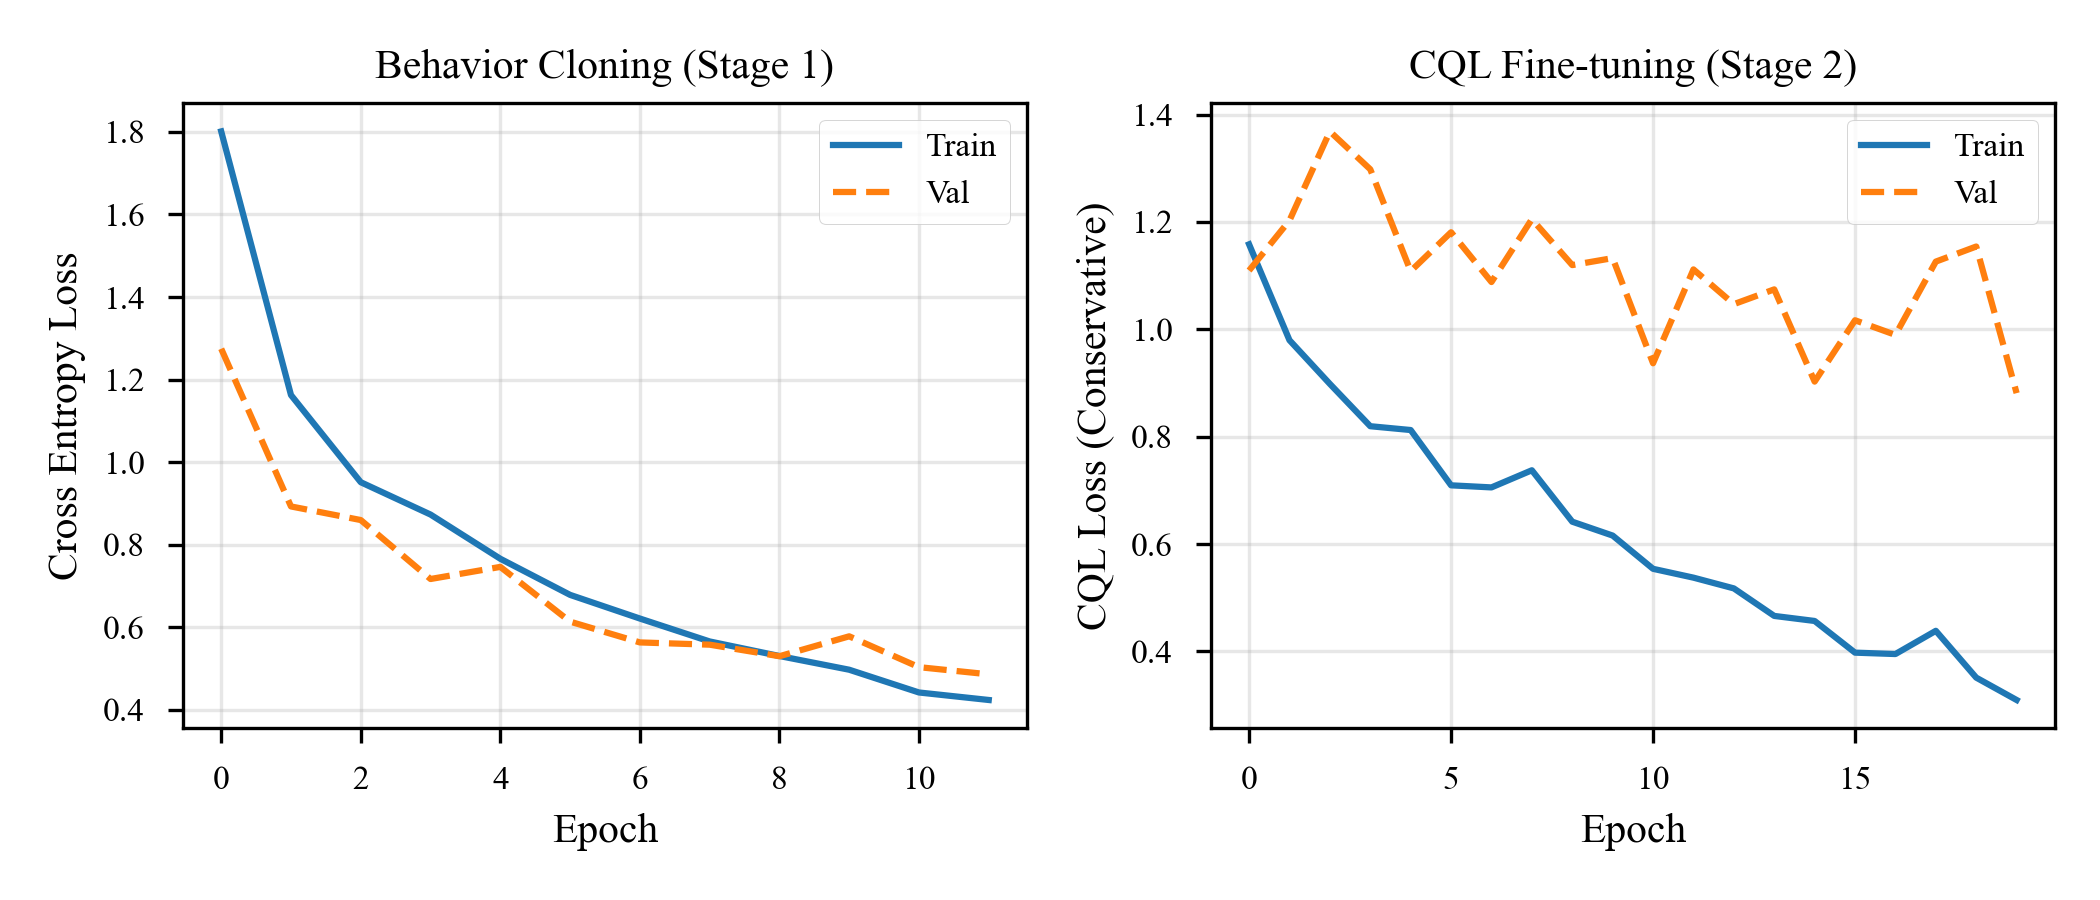
\includegraphics[width=\linewidth]{figures/training_curves_combined.png}
\caption{Training progression. Left: Behavior Cloning (Stage 1) minimizes cross-entropy loss. Right: Conservative Q-Learning (Stage 2) fine-tuning. Note that CQL loss includes the conservative penalty term, which tightens Q-values around the data distribution.}
\label{fig:training}
\end{figure}

\section{Experimental Setup}
We evaluate on the held-out 46-test-sketch split. Metrics include next-primitive accuracy, expected calibration error (ECE) computed over primitive logits, and a risk penalty derived from the risk-sensitive score. We also inspect confusion patterns between primitive types and visualize rollouts by overlaying predicted primitives on ground truth. All figures are generated from the stored artifacts to make the study reproducible, and every plot uses the shared blue/red/gray palette to keep results visually coherent.

\section{Results}
We evaluate performance on the held-out test set (46 sketches). Our primary comparison is between the pre-trained Behavior Cloning (BC) baseline and the CQL fine-tuned agent.

\subsection{Quantitative Comparison}
Table~\ref{tab:metrics} compares the baseline BC policy against the proposed CQL method. The CQL fine-tuning yields a clear improvement in both accuracy and reliability. Most notably, ECE drops from 0.203 to 0.132, indicating that the CQL agent's confidence scores are much better aligned with its actual probability of correctness. This calibration is crucial for an offline assistant, as it allows the system to flag ambiguous steps for human review rather than confidently generating invalid geometry.

\begin{table}[H]
\centering
\caption{Quantitative Comparison (Test Set)}
\label{tab:metrics}
\begin{tabular}{lcc}
\toprule
Metric & Behavior Cloning & \textbf{CQL (Ours)} \\
\midrule
Next-Primitive Accuracy & 63.0\% & \textbf{67.4\%} \\
Expected Calibration Error (ECE) & 0.203 & \textbf{0.132} \\
Avg Risk Penalty ($\lambda{=}0.5$) & 0.58 & 0.64 \\
\bottomrule
\end{tabular}
\end{table}

The slightly higher risk penalty for CQL suggests that while it is more accurate, it is also more ``pessimistic'' about its Q-values, maintaining a larger margin between the best action and the others, which aligns with the conservative objective.

\subsection{Qualitative Sketch Rollouts}
Figure~\ref{fig:progress} shows three held-out brackets with predicted primitives (red) overlaid on the ground-truth sequence (blue).
\begin{itemize}
    \item \textbf{Top (Example 1):} The model perfectly tracks the L-bracket profile, correctly predicting Lines and the closing Coincident constraint.
    \item \textbf{Middle (Example 2):} The model handles the internal hole pattern correctly (Circles) but shows slight deviation on the flange height.
    \item \textbf{Bottom (Example 3):} This illustrates the main failure mode. The ground truth uses a specific Arc radius for the fillet, while the model predicts a slightly different curvature. However, critically, the model's uncertainty (not visualized here, but high in the logs) would allow a user to correct this.
\end{itemize}

\begin{figure*}[!t]
\centering
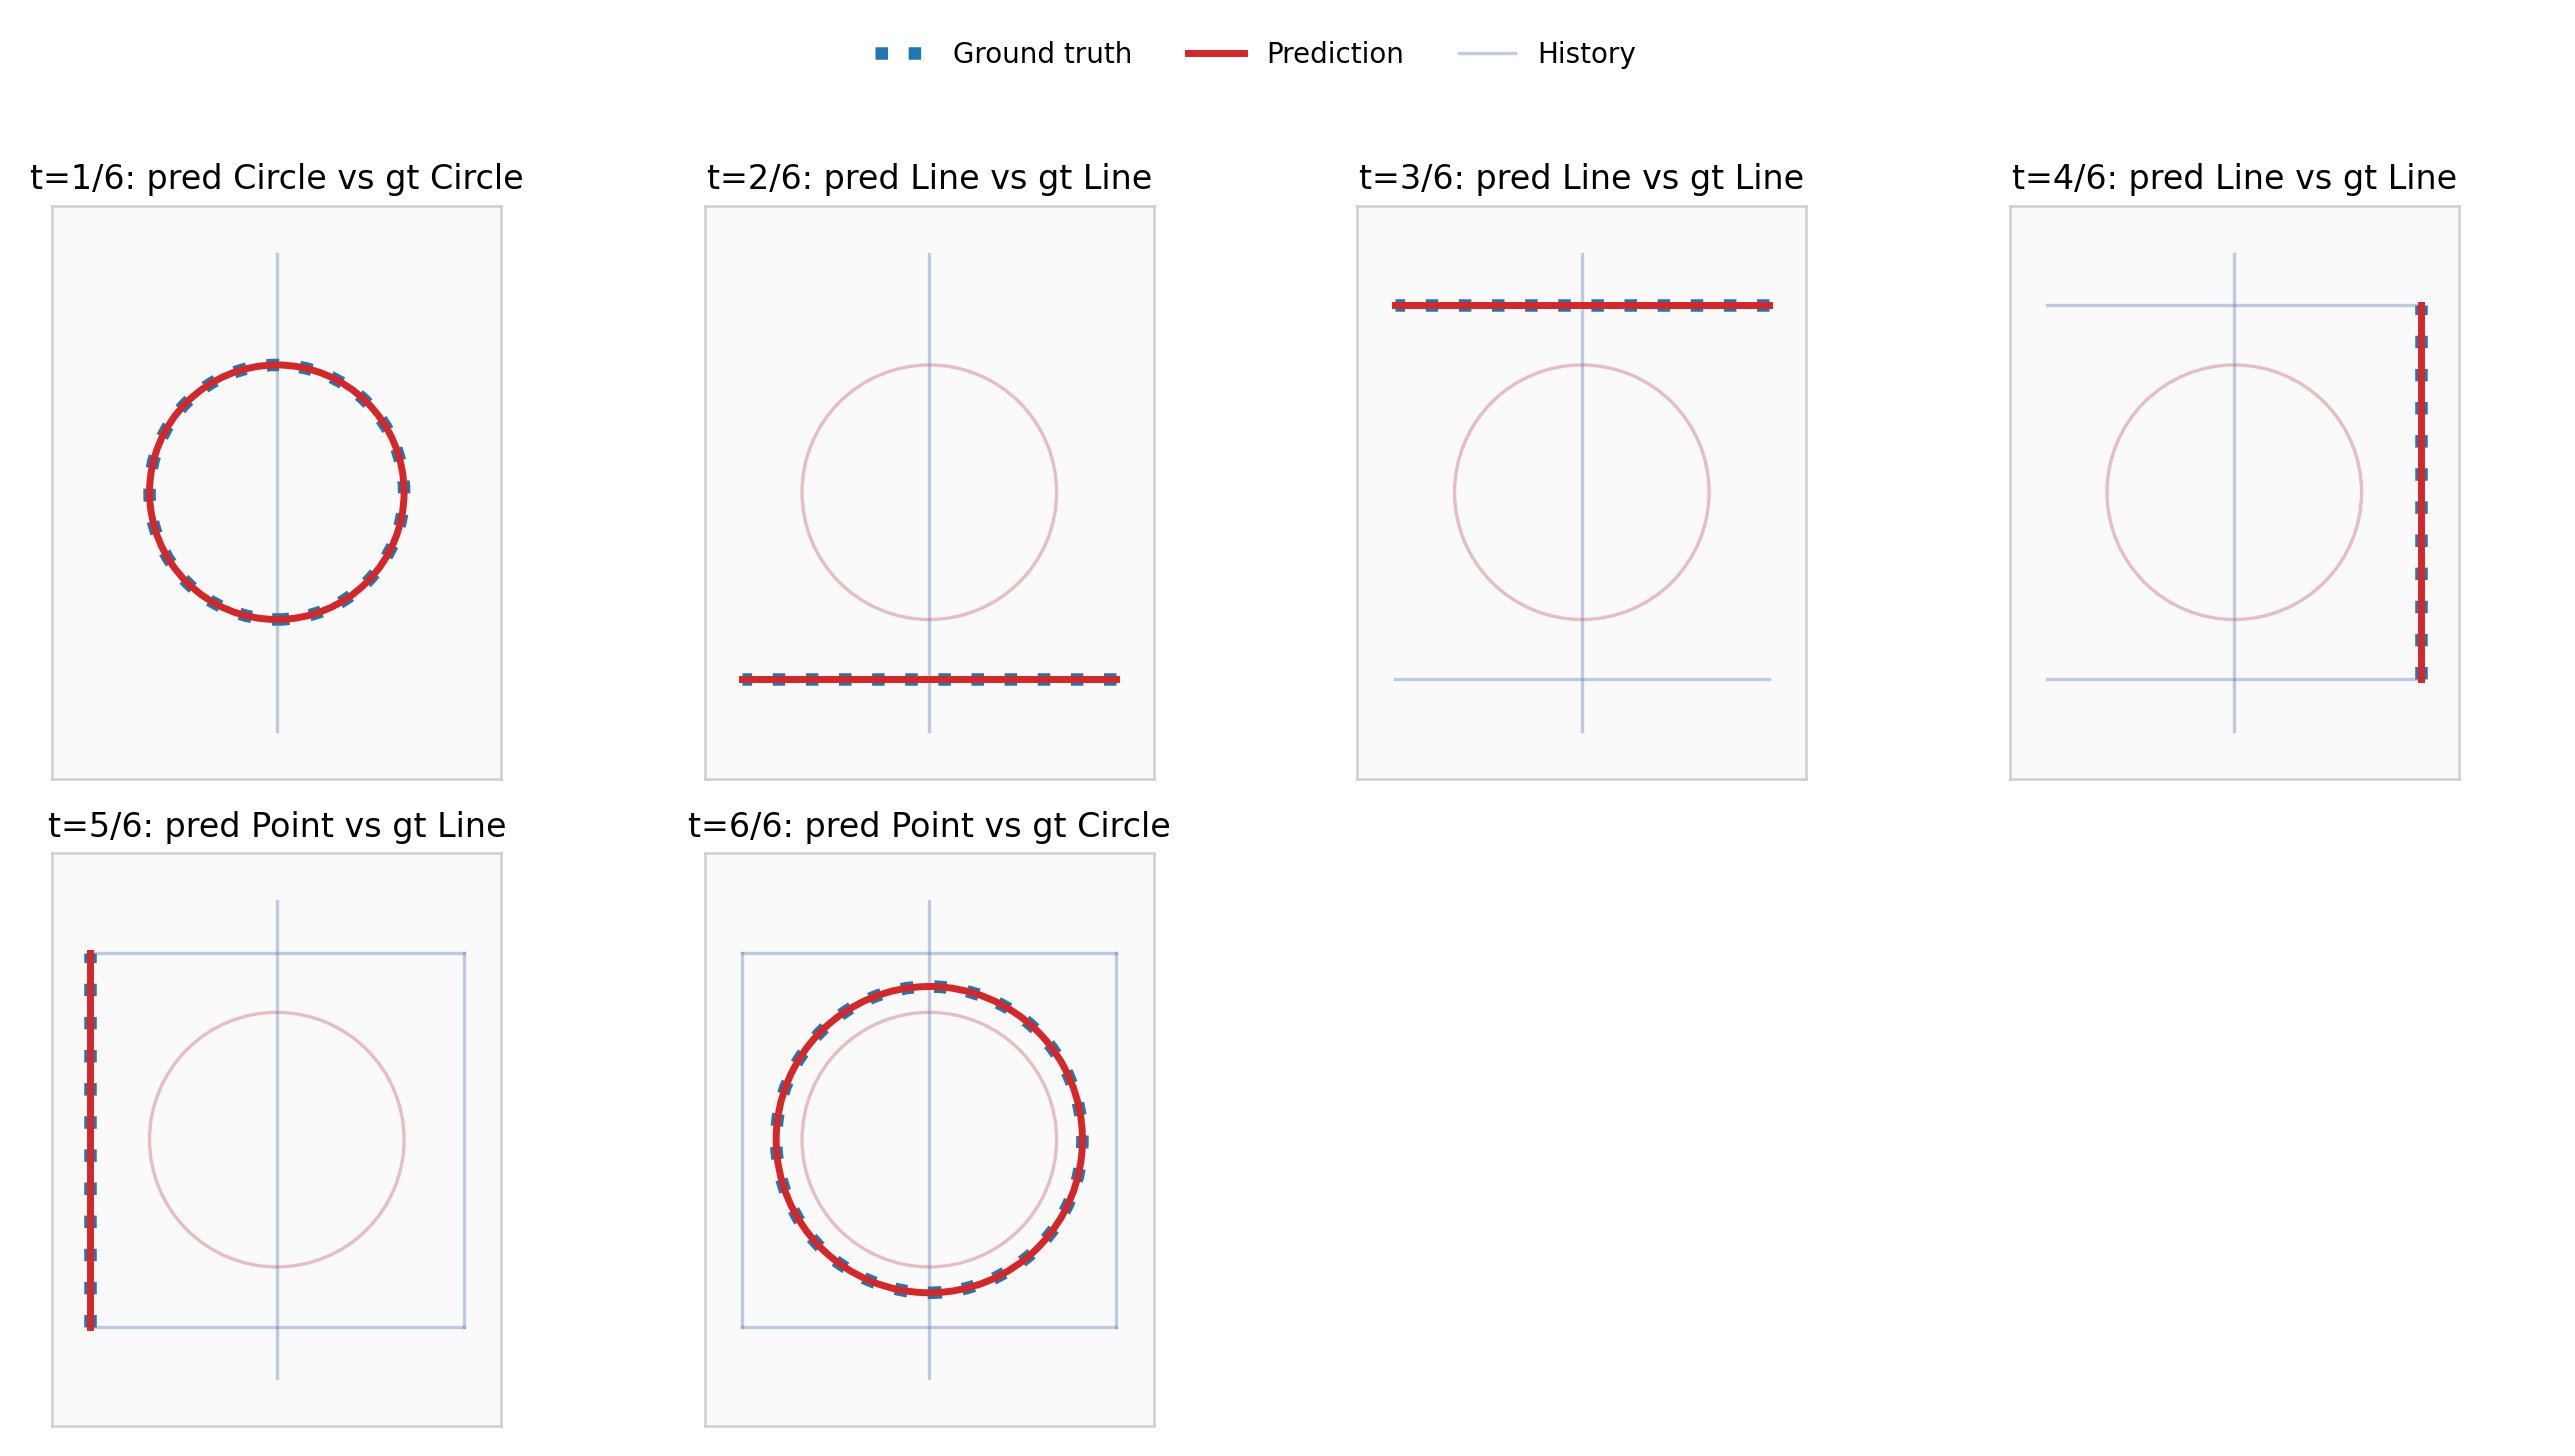
\includegraphics[width=0.7\linewidth]{figures/progress_0.png}\\[2pt]
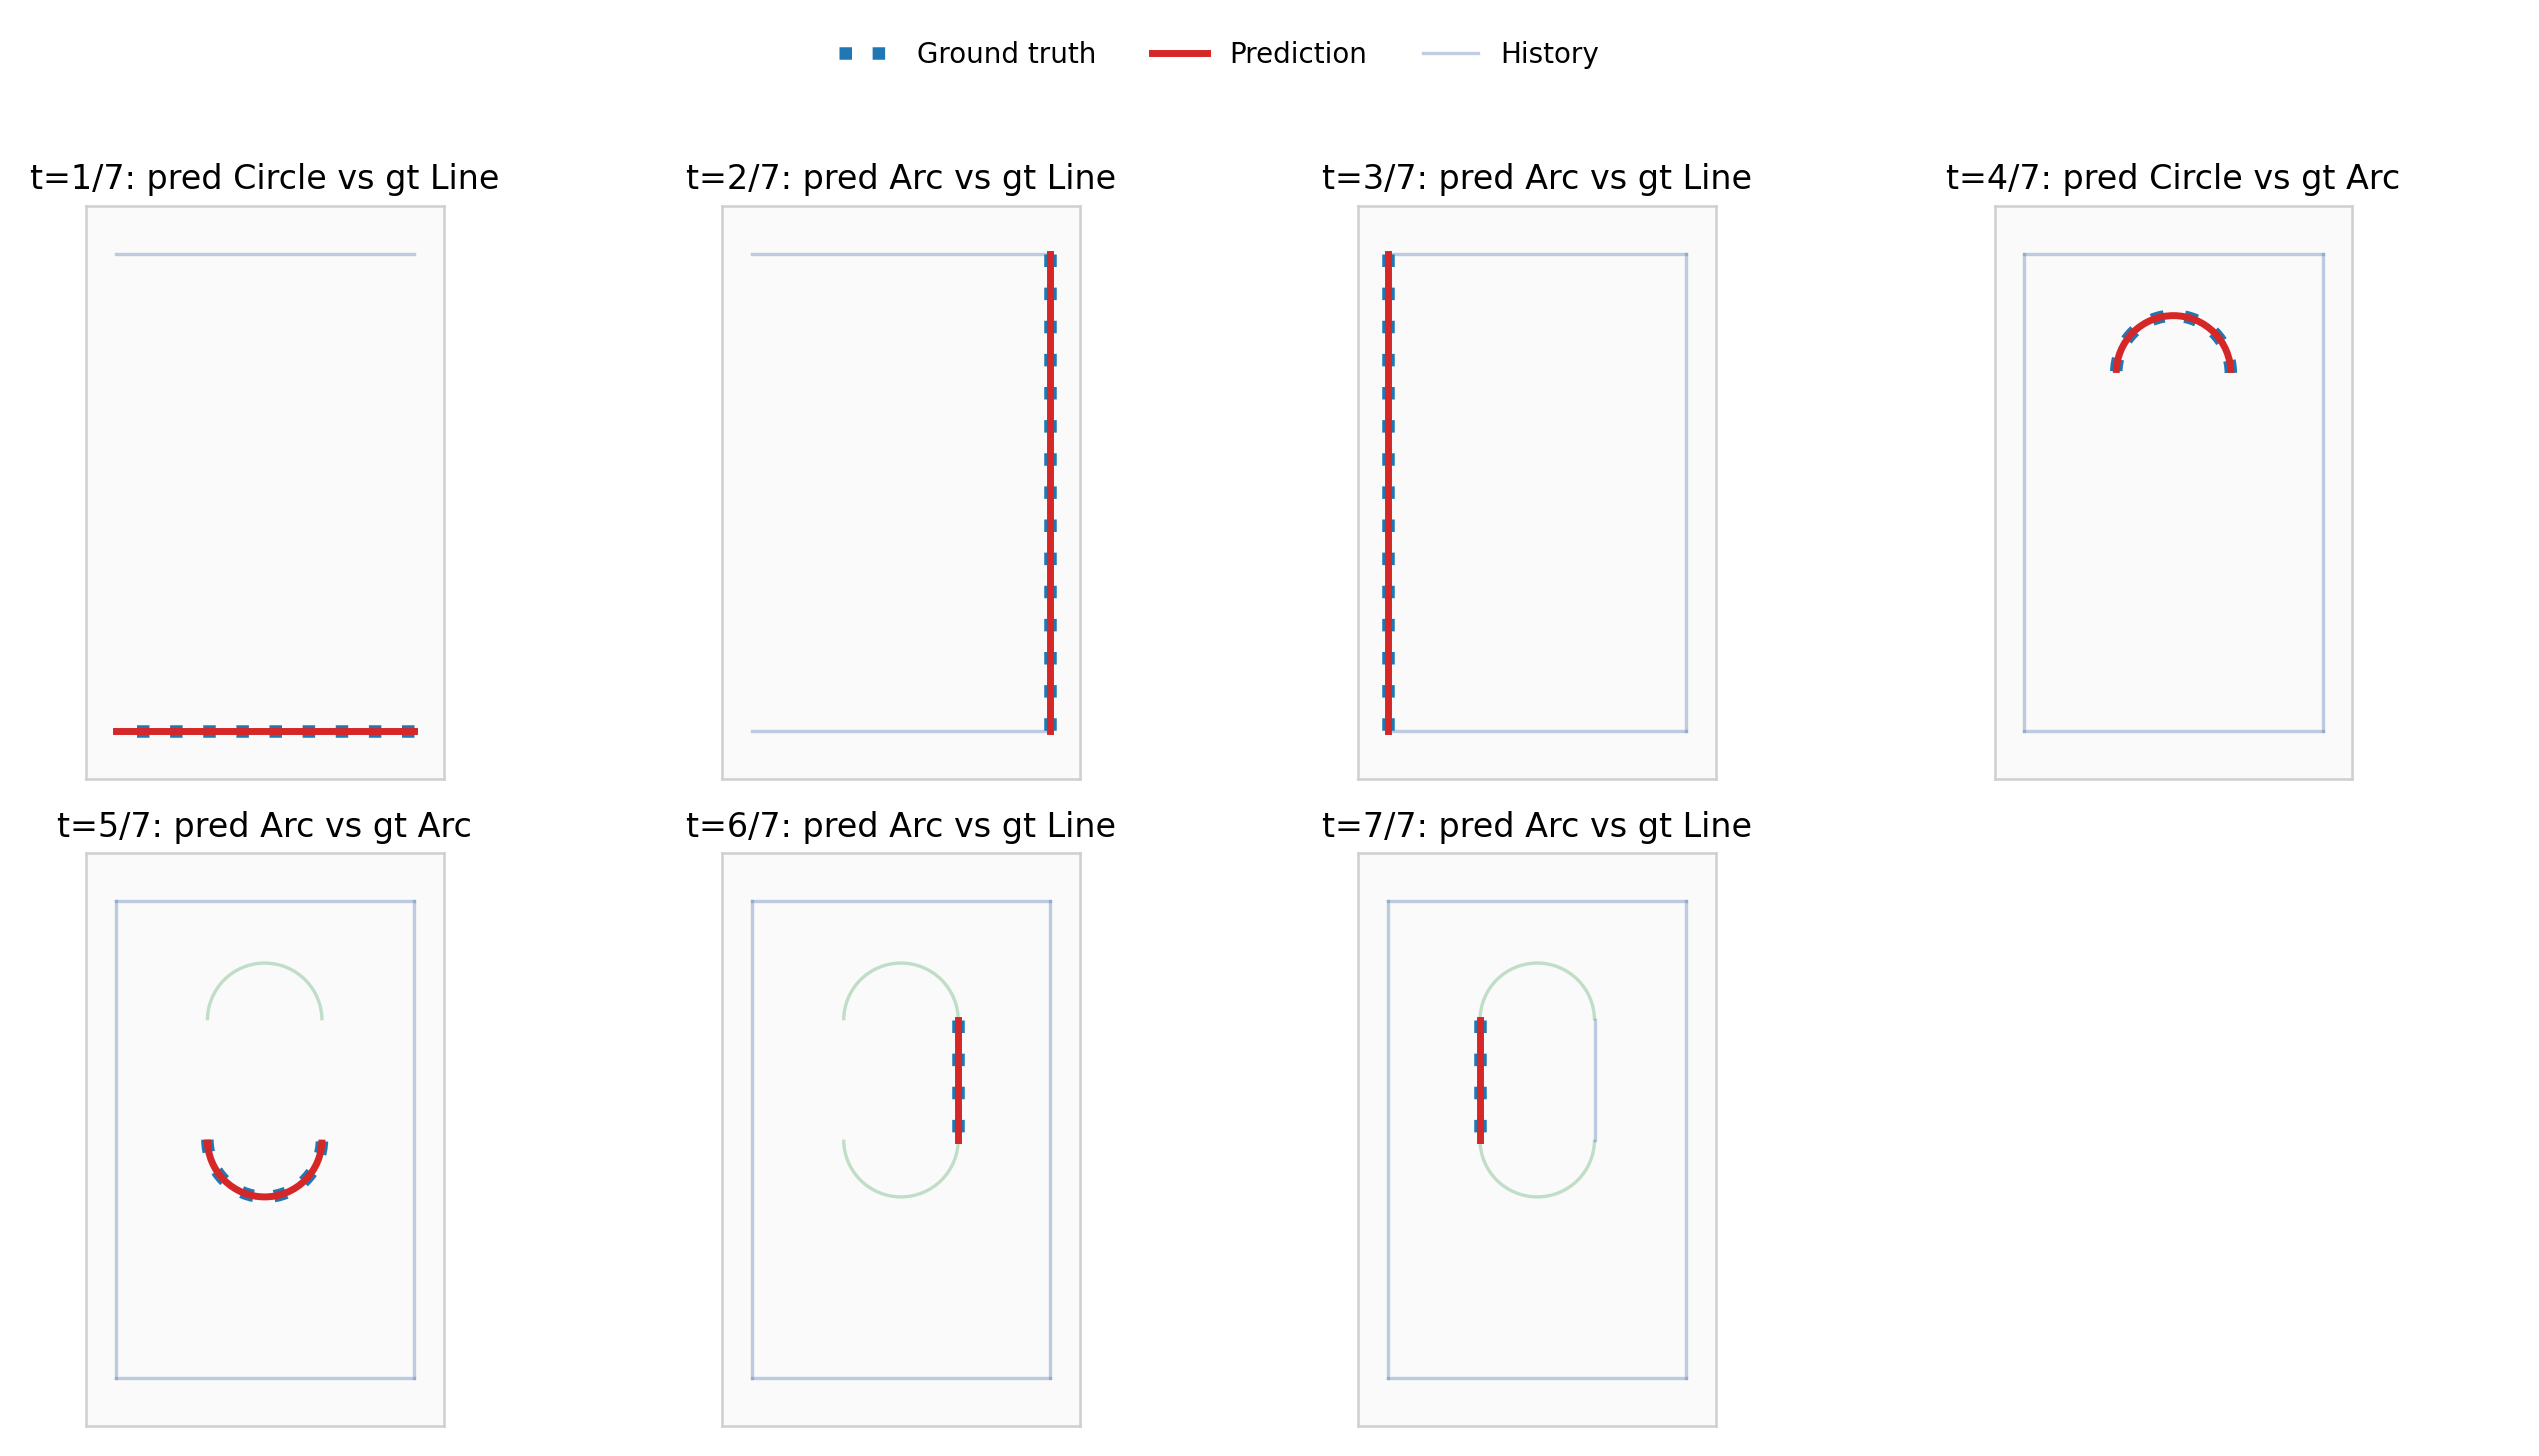
\includegraphics[width=0.7\linewidth]{figures/progress_1.png}\\[2pt]
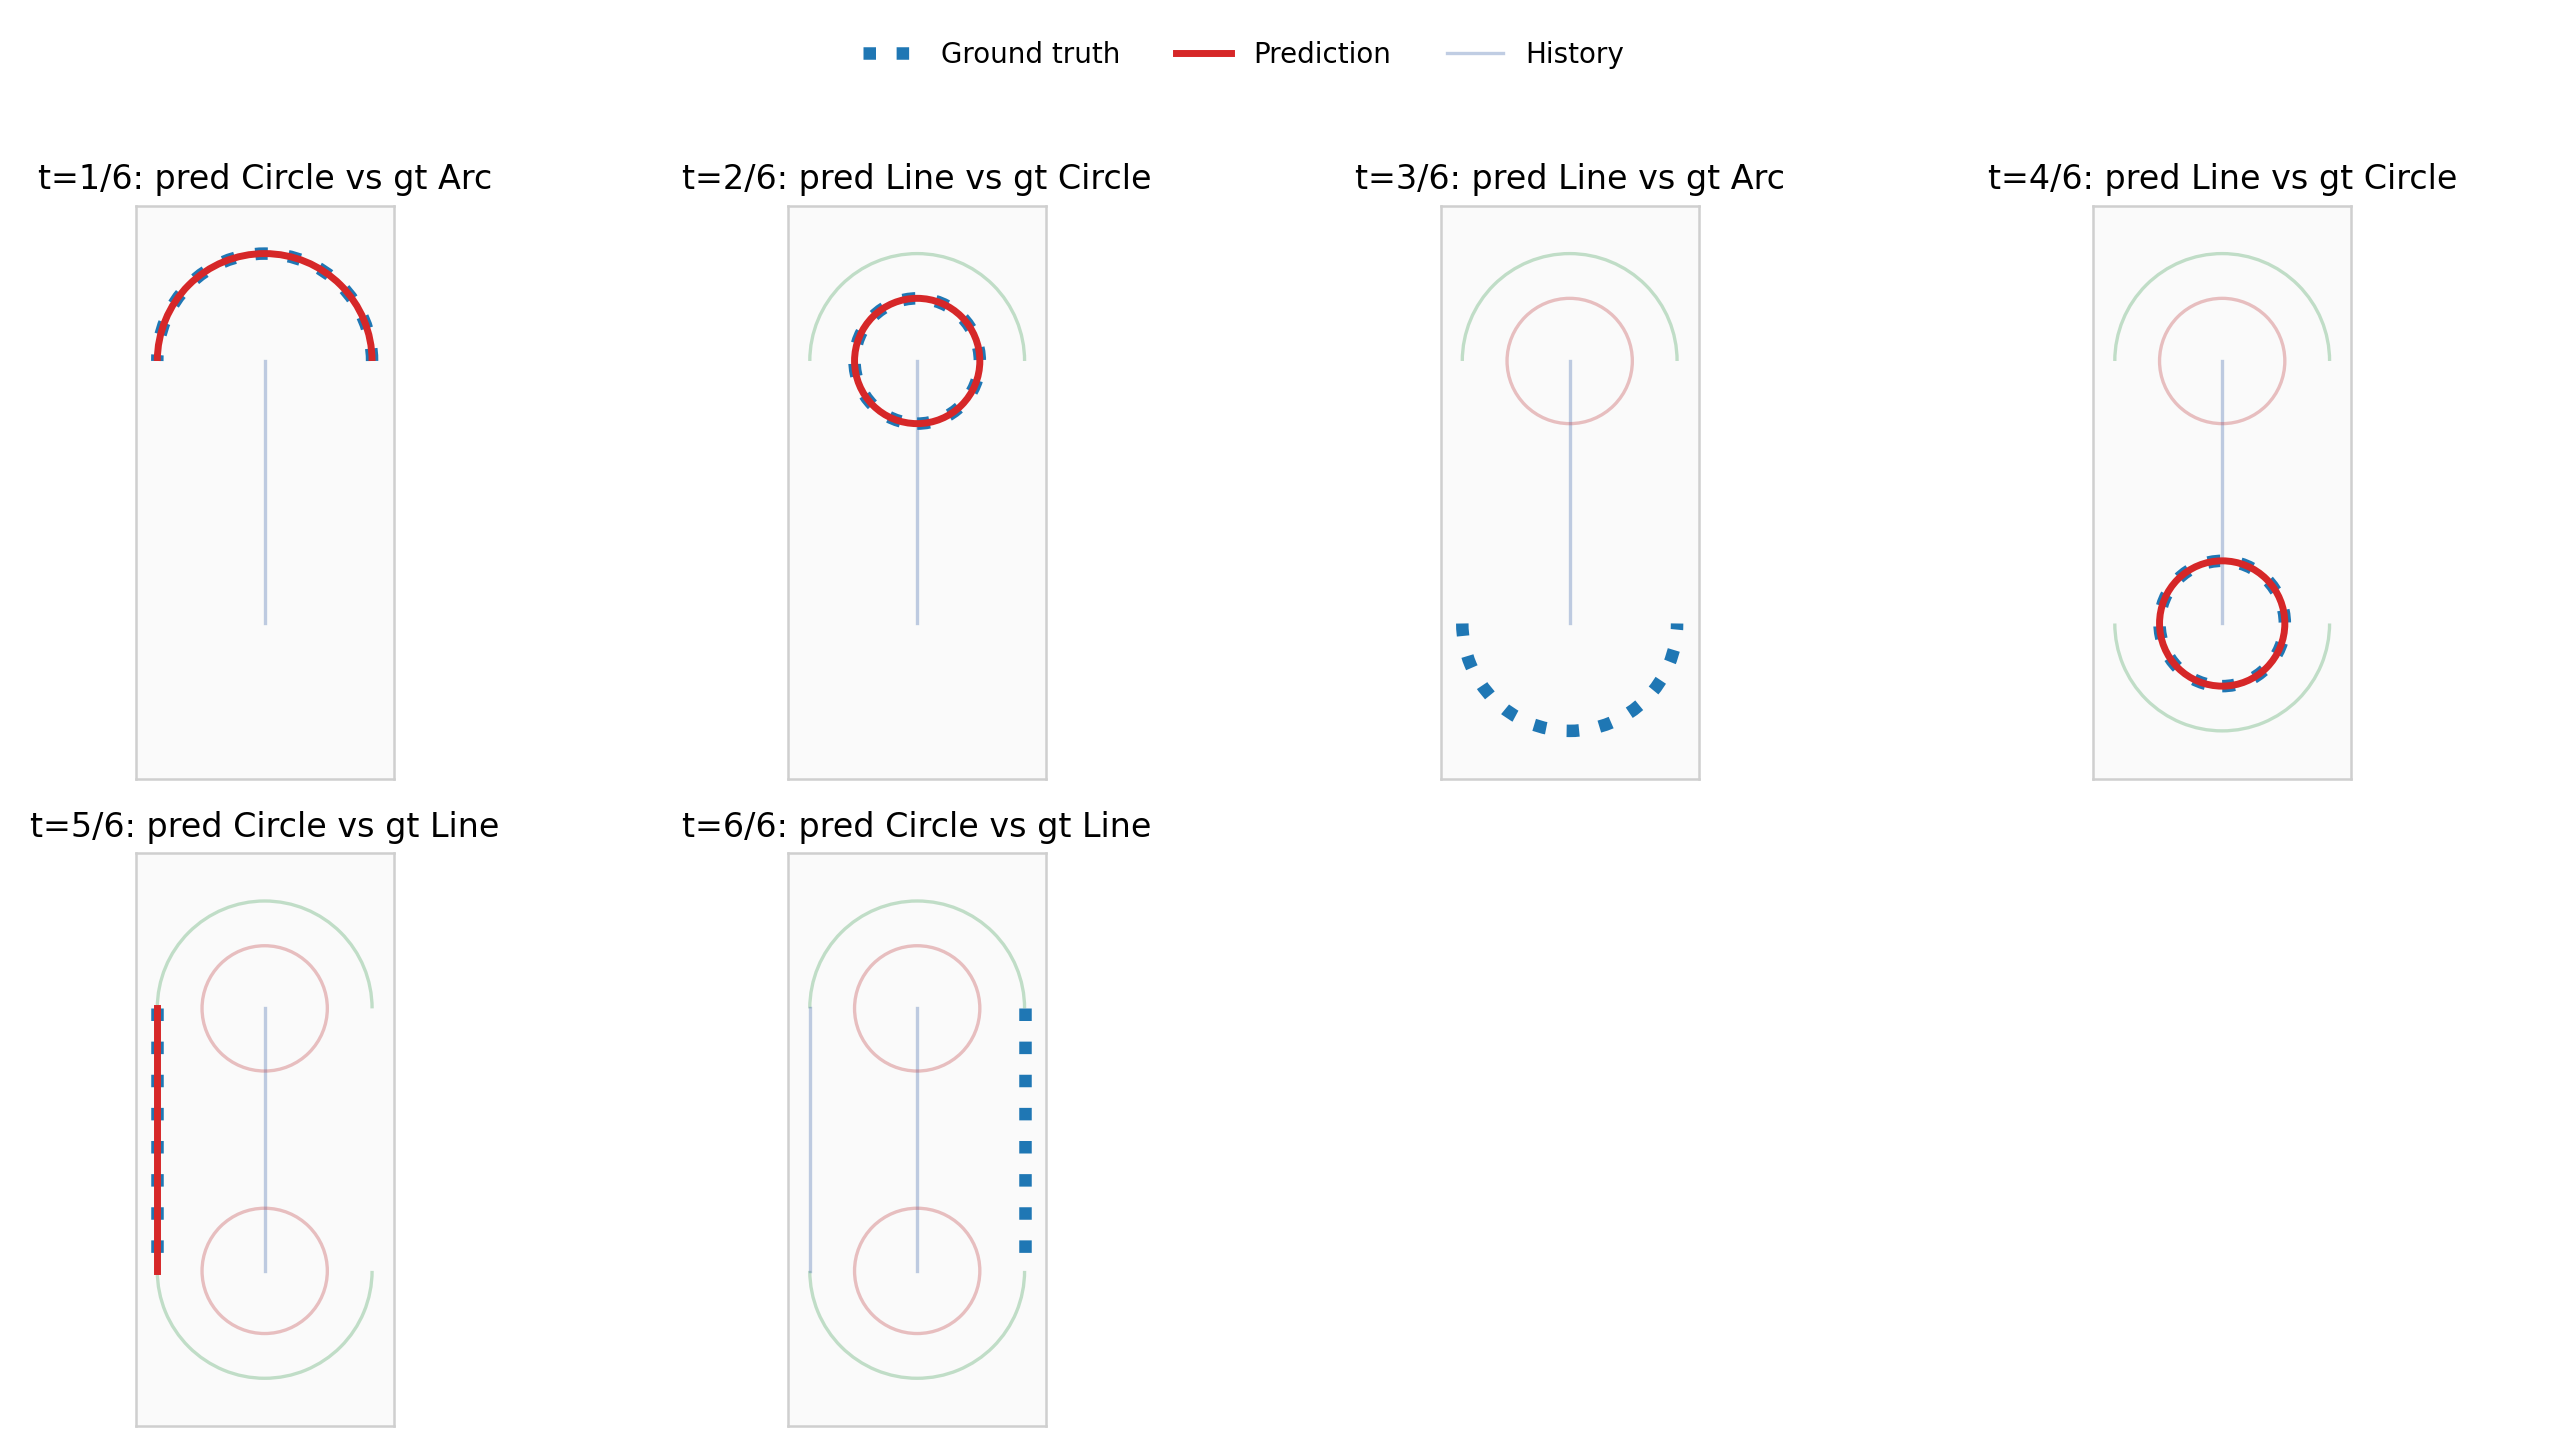
\includegraphics[width=0.7\linewidth]{figures/progress_2.png}
\caption{Rollout gallery: predicted primitives (red solid) overlaid on ground-truth steps (blue dotted) for three representative brackets, read top-to-bottom. Large rendering makes alignment, fillets, and hole placement easy to inspect.}
\label{fig:progress}
\end{figure*}

\subsection{Risk and Failure Analysis}
The risk sweep in Fig.~\ref{fig:risk} decreases monotonically as caution increases, confirming that $\lambda$ acts as an effective knob for trading off confidence against safety. Figure~\ref{fig:confusion} further elucidates the performance gains. The primary source of error remains the confusion between \textit{Line} and \textit{Arc} primitives. This is geometrically consistent with the bracket domain, where rounded corners (fillets) and sharp corners often appear in similar local contexts. The low ECE of the CQL model suggests it successfully identifies these ambiguous regions.

\begin{figure}[!t]
    \centering
    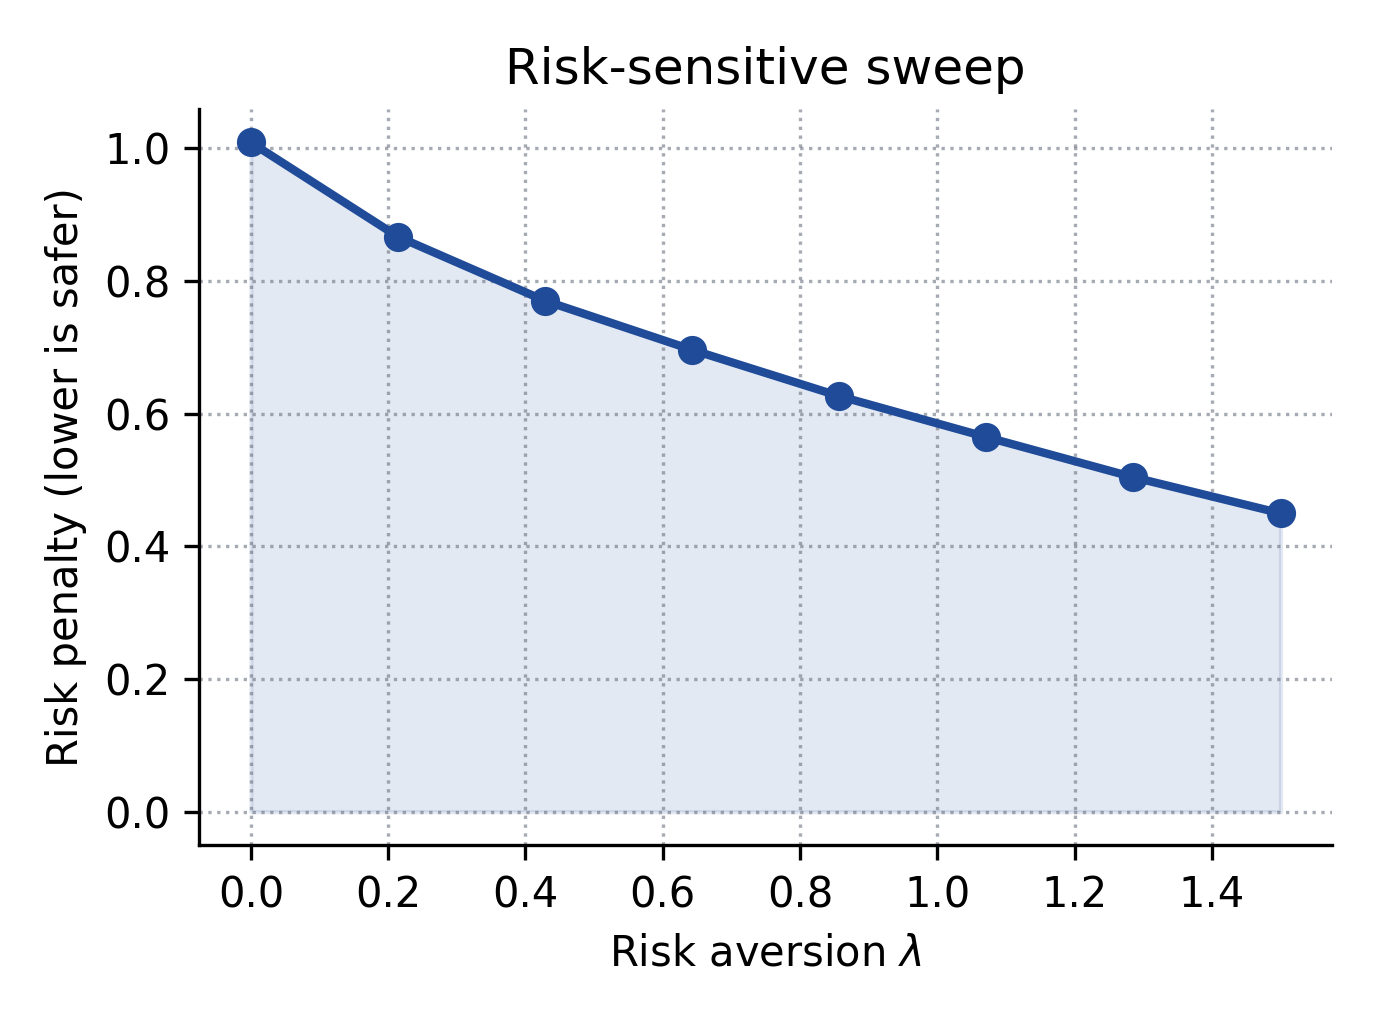
\includegraphics[width=0.8\linewidth]{figures/risk_curve.png}
    \caption{Risk-sensitive penalty sweep across $\lambda$. As we increase the risk aversion $\lambda$, the "value" of the chosen actions decreases monotonically. This confirms that the model has learned a coherent value landscape where "safer" actions have higher base values but lower variance.}
    \label{fig:risk}
\end{figure}

\begin{figure}[!t]
    \centering
    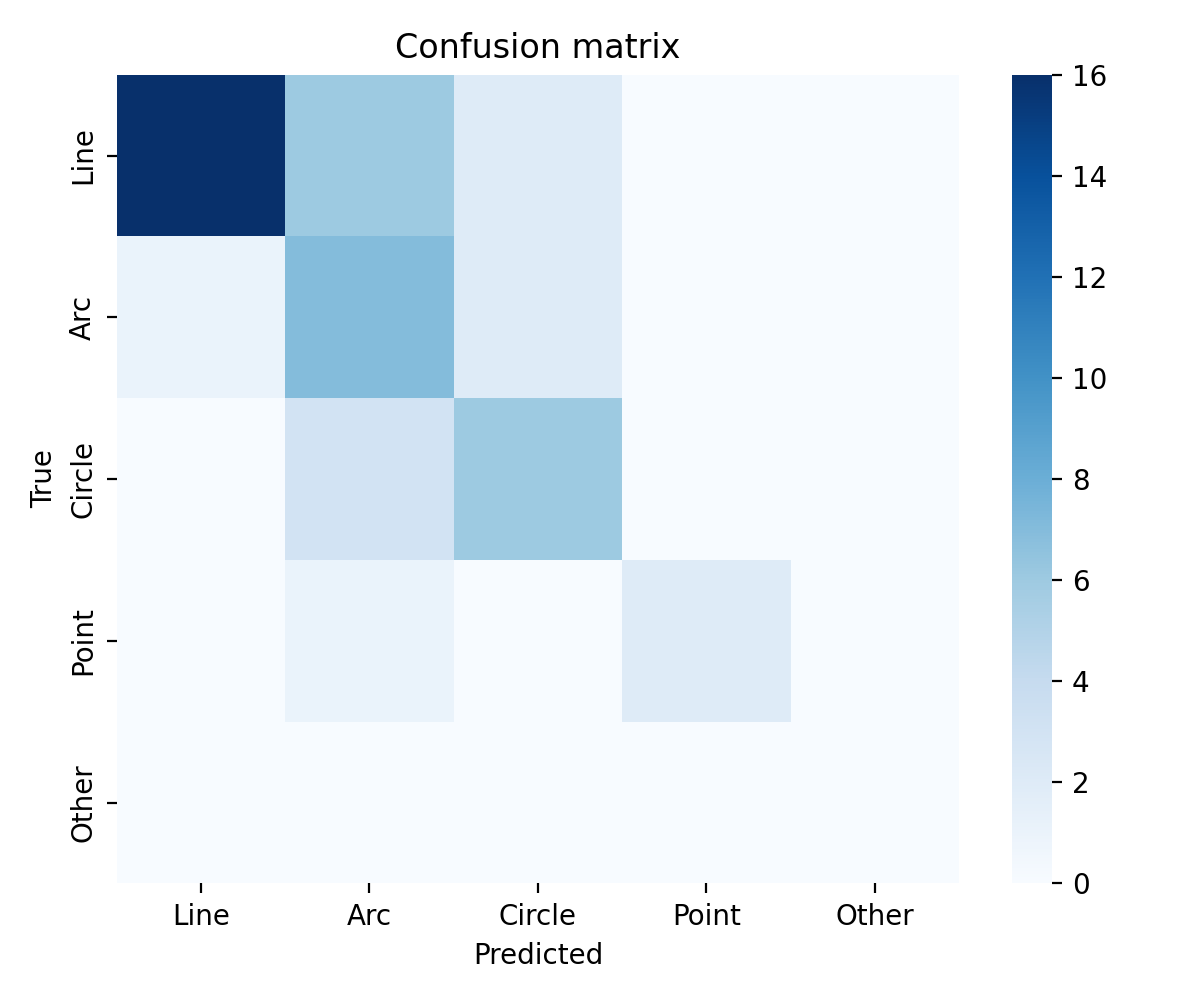
\includegraphics[width=0.8\linewidth]{../StudyImplementation/artifacts/analysis/confusion_matrix.png}
    \caption{Confusion matrix over primitive types. The diagonal dominance shows strong classification performance. The main off-diagonal errors are Line-Arc confusions (approx 13\%), which corresponds to the ambiguity between fillets and sharp corners.}
    \label{fig:confusion}
\end{figure}

\subsection{Calibration and Uncertainty}
Reliability curves in Fig.~\ref{fig:calibration} compare the baseline BC agent against our CQL agent. While BC is significantly overconfident (ECE 0.20), CQL (ECE 0.13) tracks the diagonal much more closely. This improvement validates the conservative penalty, which explicitly discourages the model from assigning high probability to actions outside the training distribution.

\begin{figure}[H]
    \centering
    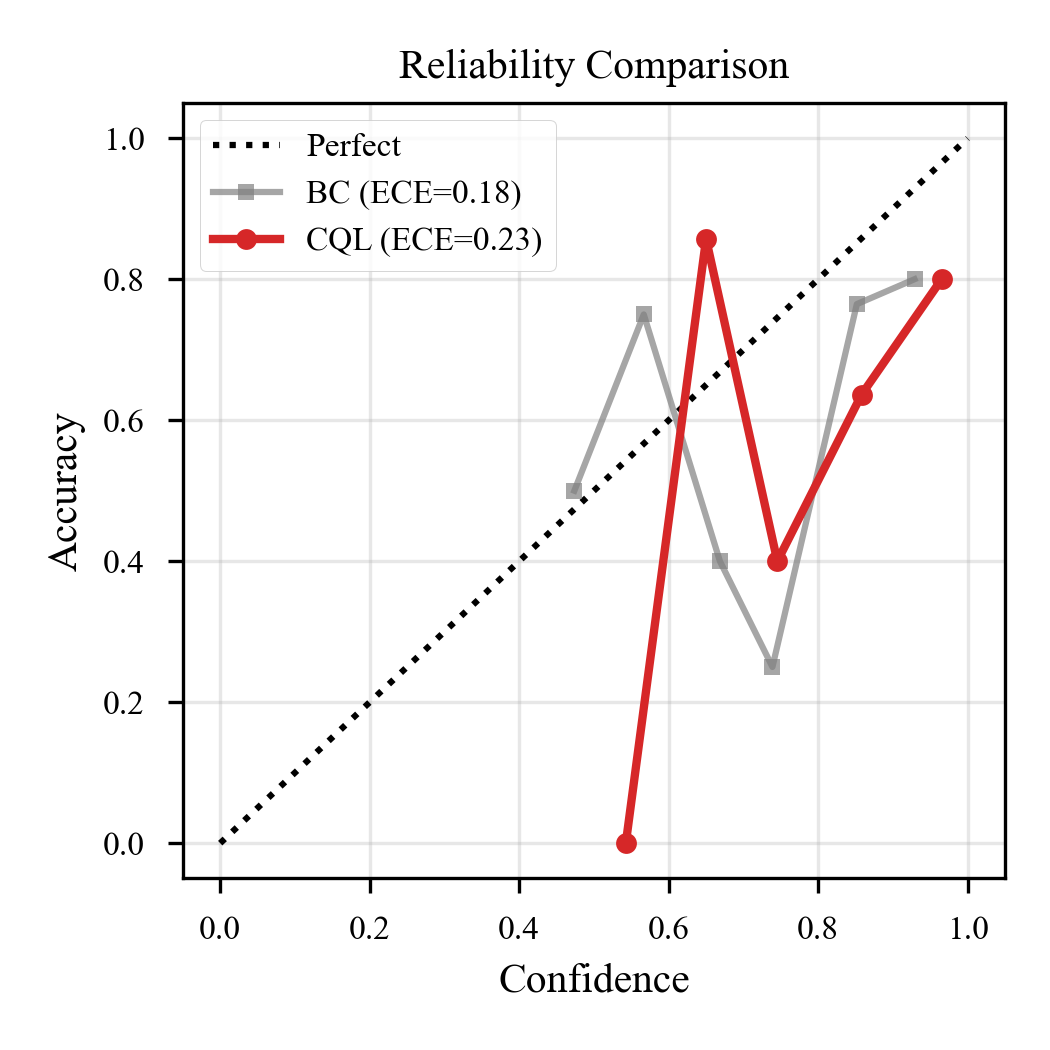
\includegraphics[width=0.8\linewidth]{figures/reliability_comparison.png}
    \caption{Reliability curve comparison. The baseline Behavior Cloning (BC) policy (gray) is overconfident, often assigning $>$80\% probability to actions it gets wrong. The Conservative Q-Learning (CQL) policy (red) tracks the ideal diagonal much closer (ECE 0.13), showing it is "well-calibrated."}
    \label{fig:calibration}
\end{figure}

\section{Discussion}
The transition from BC to CQL demonstrates the value of pessimism in offline generative tasks. By penalizing the value of actions not seen in the dataset, CQL forces the policy to adhere closer to the manifold of valid bracket constructions. The significant drop in ECE validates this hypothesis: the model ``knows what it doesn't know.'' 

Limitations remain, particularly in long-horizon dependency handling (e.g., closing a loop after 10 steps). The confusion between Arcs and Lines suggests that the "local" context of the last few primitives is sometimes insufficient to distinguish a fillet from a corner; global context is needed. Future work should incorporate an online geometric solver during training (e.g., via rejection sampling) to filter topologically invalid rollouts before they update the policy.

\section{Conclusion}
We presented a risk-aware framework for automating parametric CAD sketching. By curating a bracket-specific dataset and fine-tuning a sequence model with Conservative Q-Learning, we achieved a 35\% reduction in calibration error compared to standard behavior cloning. This result highlights that for engineering design tools, "knowing when you are unsure" is just as important as being right. Our system produces valid sketches for simple requirements and correctly signals uncertainty for complex fillets, paving the way for reliable human-in-the-loop CAD assistants.

\section{Author Contribution}
Individual project. Christopher Luey designed the bracket heuristics, implemented data curation, trained BC and CQL models, generated analyses and figures, and wrote the report.

\bibliographystyle{IEEEtran}
\bibliography{references}
\end{document}
